\section{HaCWB}

Nesta secção, será explicado o objectivo desta ferramenta, bem como o modo de utilização. Todas 
as opções permitidas serão explicadas, bem como o modo de funcionamento.

\subsection{Descrição da Ferramenta}

Como já foi dito anteriormente, neste momento esta ferramenta apenas manipula processos e permite 
criar grafos de transição. Assim, recebendo como parâmetro de entrada um ficheiro em CCS contendo 
processos, o \textit{parser} lê-os, e coloca-os numa estrutura de dados intermédia, mais concretamente, 
uma lista de pares da forma (Nome do Processo , Processo), para posterior manipulação.

\subsection{Utilização do HaCWB}

Para melhor compreender e utilizar o hacwb, passamos à descrição de todas as opções disponíveis, e 
ainda o seu modo de funcionamento. Serão apresentados ainda alguns breves exemplos de utilização.

\begin{itemize}
\item \textit{-h} - Opção de ajuda. Quando incluida nas opções, é imprimido um texto de ajuda, com 
todas as opções da ferramenta.\\
Segue-se um exemplo da invocação da ferramenta com esta opção:\\
\begin{verbatim}
/src/bin$ ./hacwb -h

HaCWB - A Haskell tool to manipulate processes.
Usage: hacwb options ...

List of options:

  -H, -h                    --help           
                           output a brief help message
  -L file_in, -l file_in    --load=file_in   
                           specify input file
  -S file_out, -s file_out  --save=file_out  
                           save transition graph
  -G, -g                    --graph          
                           generate transition graph
  -F, -f                    --save           
                           generate multiple files 
                           with transition graphs


For more information see README file.
\end{verbatim}
\item \textit{-g} - Para criar grafos de transição a partir de um ficheiro de \textit{input}, é necessário 
incluir esta opção na ferramenta.
\item \textit{-l} - Esta opção requer argumento. Assim, dado um ficheiro de entrada em CCS, o hacwb 
faz o \textit{parsing} do ficheiro, e grava para uma estrutura de dados intermédia os processos lidos.\\
Para invocar o hacwb com esta opção: \textit{hacwb -g -l"fin"}.\\
Note-se que invocando desta maneira o hacwb, todo o \textit{output} será redireccionado para o monitor.\\
De seguida, mostra-se um exemplo de um ficheiro de \textit{input}, aceite pelo hacwb:\\
\begin{verbatim}
P1 = (c.d.0 + w.0);

P2 = new {a} (a.0 | ~a.b.0);
\end{verbatim}
\item \textit{-s} - Para guardar os grafos de transição criados apenas num ficheiro, basta invocar a ferramenta 
com esta opção seguida de um argumento (nome do ficheiro de saída sem extenção), para que todos os grafos de 
transição possam ser guardados (codificados em GraphViz), para posteriormente o utilizador vizualizar.\\
Para invocar o hacwb com esta opção: \textit{hacwb -g -l"fin" -s"fout"}.\\
Após invocar o hacwb com o ficheiro de entrada referido no ponto anterior, e depois de gerar o respectivo 
\textit{postscript} através da ferramenta \textit{dot} incluida no GraphViz, obtemos os seguintes grafos de 
transição:

\begin{figure}[!htb]
\begin{center}
\label{fig:tg}
\resizebox{.35\textwidth}{!}{\includegraphics{out.ps}}
\caption{Grafo de transição referente ao ficheiro de entrada apresentado anteriormente.}
\end{center}
\end{figure}

\item \textit{-f} - Por fim, para guardar cada processo lido do ficheiro de entrada independentemente, utiliza-se 
a opção -f. Desta forma, sao criados \textit{n} ficheiros (com \textit{n} número de processos, e em que o nome 
do ficheiro é o inteiro respectivo).\\
Para invocar o hacwb com esta opção: \textit{hacwb -g -l"fin" -f}.\\
O resultado desta invocação, para i ficheiro de entrada anterior, são 4 ficheiros \textit{dot}, com os grafos de 
transição separados por ficheiros.
\end{itemize}

\subsection{Estruturas de dados criadas para definir Processos}

Aqui, apresentam-se as estruturas de dados mais importantes criadas ao longo da realização deste trabalho prático, 
para definir processos e grafos de transição.\\
Em primeiro ligar é necessário definir processos. Para isso foi criado o tipo \textit{Process}, com todos os construtores 
necessários. Um desses construtores, mais concretamente o consrutor \textit{NameP}, foi criado para dar um nome a um processo, 
para assim permitir que processos de invoquem mutuamente. Segue-se o tipo de dados:\\

\begin{verbatim}
data Process a = Or (Process a)  (Process a)
                | Paralel (Process a) (Process a)
                | Dot (Action a) (Process a)
                | Zero 
                | New [a] (Process a)
                | NameP String
\end{verbatim}

Depois de definir processos, torna-se necessário definir Acções. Tomamos como acções a acção de sincronização \textit{Tau}, 
bem como as variáveis e os seus complementares:\\

\begin{verbatim}
data Action a = Var a 
                | Comp a 
                | Tau
\end{verbatim}

Quando lêmos um ficheiro de entrada, gravamos o conteúdo do ficheiro CCS numa estrutura intermédia, chamada \textit{LstProcesses}, 
definida mais a baixo, para atribuir a cada processo um nome:\\

\begin{verbatim}
type LstProcesses a = [(String, Process a)]
\end{verbatim}

Por fim, para definir grafos de transição foi definido um tipo de dados, similar a \textit{Rose Tree}, contendo no nodo 
o processo e de seguida uma lista de todas as possíveis derivações:\\

\begin{verbatim}
data TransG a p = Node p [(a,TransG a p)]
\end{verbatim}

Para além destas estruturas de dados, foram criadas mais estruturas auxiliares, das quais destacamos a estrutura de estado, 
utilizada na avaliação de processos (possívelmente infinitos):\\

\begin{verbatim}
type Stt a = (Int, Path a, LstTrees a)
\end{verbatim}

Em que:\\

\begin{verbatim}
type Path a = [(Action a, Process a)]

type LstTrees a = [(Process a, Path a)]
\end{verbatim}

